\subsection{Was wird getestet?}
\label{sec:Kap-11-1-2}

Ein großes Softwaresystem setzt sich aus Komponenten zusammen. Aus der Gesamt\-spe\-zi\-fi\-ka\-tion muss eine Spezifikation für diese Komponenten folgen, so dass aus der Korrektheit der Komponenten bezüglich dieser Spezifikationen und dem Zusammenspiel der Komponenten die Korrektheit des Gesamtsystems folgt. Grob unterscheidet man die Zerlegung eines Systems in Teilsysteme, die wiederum aus Modulen bestehen. Entsprechend gibt es folgende Unterscheidung (s.~Abb.~\ref{fig:puzzle_testen}):

% Abbildung händisch verschoben.
% Hier gehört die Abbildung {fig:puzzle_testen} eigentlich hin.

\begin{itemize}
	\item \textit{Komponententest} bzw. \textit{Modultest} (engl. unit test), 
	\marginline{Komponenten\-test}
	hier werden die einzelnen Komponenten bzw. Module getestet.
	\item \textit{Integrationstest} (engl. integration test), 
	\marginline{Integrationstest}
	hier wird das Zusammenspiel der 
	\linebreak %%% für Druck
	Module auf Teilsystemebene getestet.
	\item \textit{Systemtest} (engl. system test)
	\marginline{Systemtest}
\end{itemize}

Bis hierhin geht es beim Testen stets darum, Fehler zu finden. Tatsächlich ist dies der besondere Ehrgeiz der Tester, und sie sind entsprechend in den Qualitäts\-verbesserungs\-prozess eingebunden. Fast kann man sagen: Wer keine Fehler findet, hat seinen Job schlecht gemacht. Irgendwann aber muss der Prozess beendet sein und das System ausgeliefert werden. Zu diesem Zeitpunkt führt man nochmal einen Test durch:

\begin{itemize}
	\item \textit{Abnahmetest} (engl. acceptance test), 
	\marginline{Abnahmetest}
	hier sollten keine Fehler mehr gefunden bzw. aufgedeckt werden, so die Hoffnung.
\end{itemize}

\begin{figure}[h!]
	\centering
	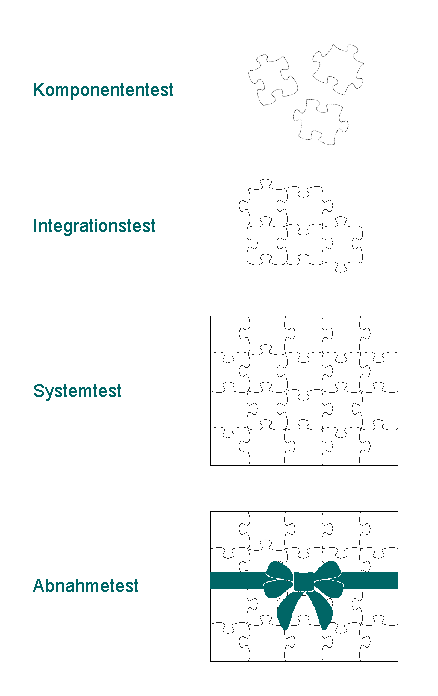
\includegraphics[width=0.55\textwidth]{Bilder/Kapitel-11/Puzzle_Testen.pdf}
	\caption[Illustration Teststrategien]{Illustration angelehnt an \cite{gli05}}
	\label{fig:puzzle_testen}
\end{figure}